%-------------------------------------------------------------------------------
\section{Preliminary Results}
%-------------------------------------------------------------------------------

% \begin{figure*}[t!]
%     \centering
%       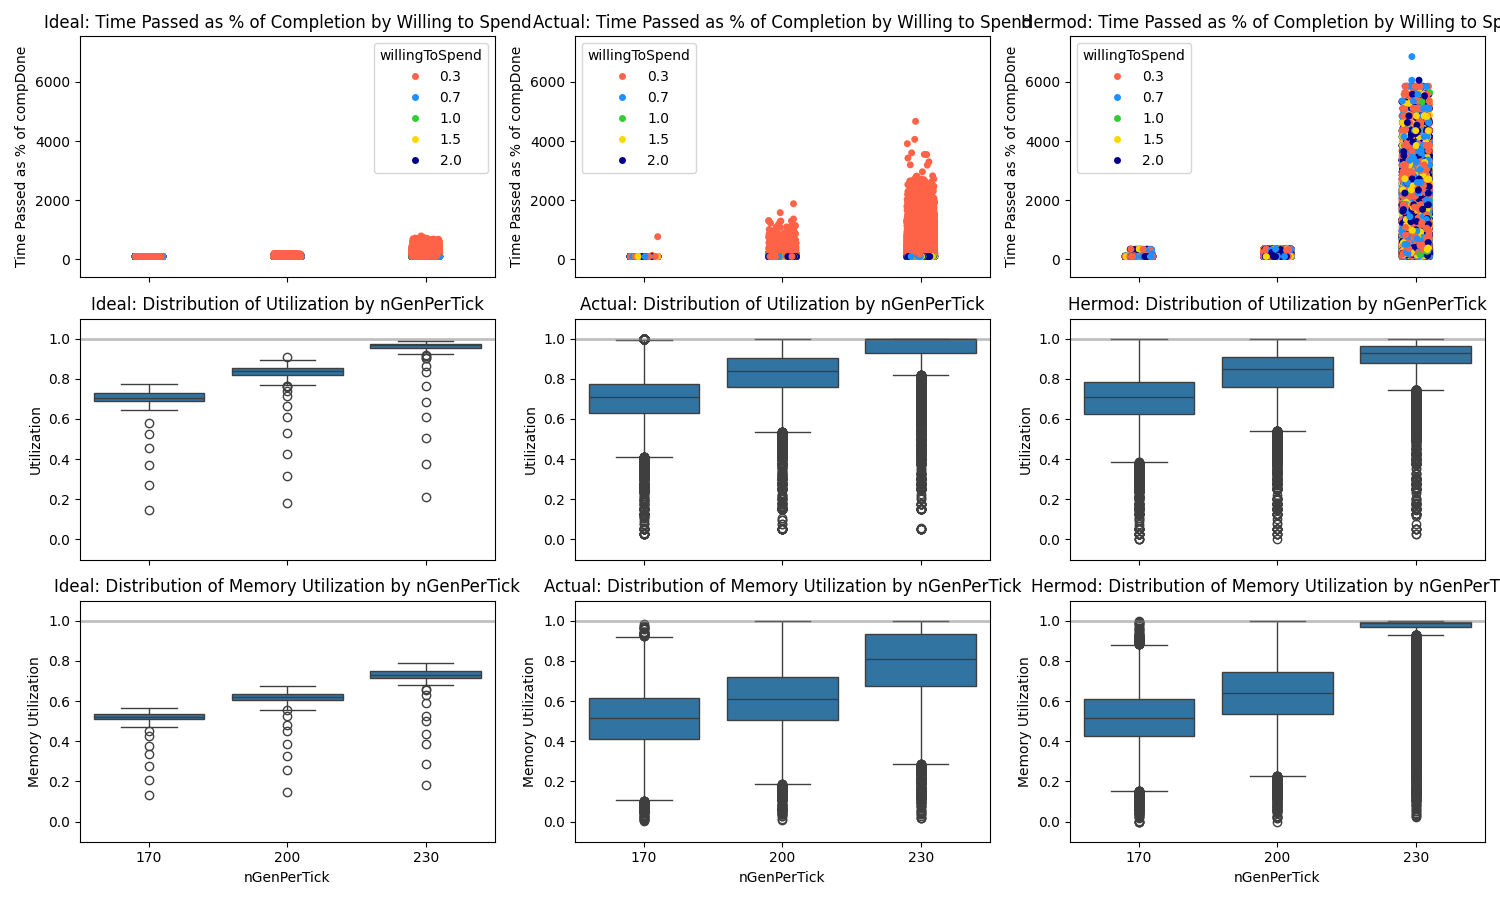
\includegraphics[width=15cm]{img/combined_res.png}
%       \caption{ a placeholder graph }
%     \label{fig:graph}
% \end{figure*}



In order to understand the case for \sys{}, we ask the following questions: 
\begin{enumerate}
    \item Are priorities good at meeting SLAs?
    \item How well do schedulers with no priority information do at meeting SLAs?
    \item Is \sys{} good at binpacking?
\end{enumerate}


To explore these questions, we built a simulator in go\cite{TODO}, which
simulates different scheduling approaches.


\subsection{Experimental Setup}

In each version of the simulator, jobs arrive in an open loop at a constant
rate. The simulator attaches three main characteristics to each job it
generates: runtime, priority, and memory usage.\ \textit{Job runtime} is chosen
by sampling from randomly generated long tailed (in this case pareto)
distribution: the relative length of the tail ($\alpha$ value) remains constant,
and the minimum value ($x_m$) is chosen from a normal distribution. This
reflects the fact that different functions have different expected runtimes
(chosen from a normal distribution), and that actual job runtimes follow long
tailed distributions (so each pareto distribution that we sample represents the
expected runtime distribution of a given function).\ \textit{Job priority} is
chosen randomly. The simulator has n different priority values, each assigned to
a fictitious price. Because functions are randomly assigned a priority, runtime
and priority are not correlated.\ \textit{Job memory usage} is chosen uniform
random between 1MB and 10GB.

When comparing two different simulated schedulers, they each are given an
identical workload and then each simulate running that workload.

The simulator makes some simplifying assumptions:
\begin{enumerate}
    \item functions are compute bound, and do not block for i/o
    \item functions use all of their memory right away
    \item communication latencies are not simulated
\end{enumerate}

\subsection{Are priorities good at meeting SLAs?}

In the end developers care about job latency, so it is important to understand
how well priorities do at reflecting and enforcing SLAs.

In order to define the desired SLA, we assign each job invocation a deadline,
and to make things simple we allow the deadline to be a function of the job's
true runtime. Simply setting the deadline to be the runtime is not realistic:
perhaps for high priority jobs that is the case, but for low priority jobs that
is not true, the reason they are low priority is because they are willing to
wait. We thus define the deadline as a function of the runtime as well as the
priority, where deadline = runtime * maxPrice/price (as if each process were
weighted by its price). We simulate an Earliest Deadline First (EDF) scheduler,
which is queuing theoretically proven to be optimal in exactly the way we
wanted: if it is possible to create a schedule where all jobs meet their
deadline, EDF will find it\cite{TODO}.

We compare the latencies observed in this EDF simulated scheduler with an
idealized version of a preemptive priority scheduler, and look at the latencies
they both get. A good result for \sys{} would show little difference between the
two: we expect the EDF version to do better, because it is both theoretically
optimal and has access to perfect information, but if the priority scheduler
does similarly then we know that it can be a good proxy for deadlines. We can
see the results in Figure~\ref{fig:graph}.\hmng{TODO do this}

\subsection{How well do schedulers without priority info do?}

This question is relevant in order to understand if we need priorities at all:
is there a scheduler that can, without having any access to information about
which jobs are important, still ensure that jobs perform well?

To explore this question, we look at how an existing state of the art research
scheduler that does not take any form of priority into account performs on the
web server's workload. We simulate Hermod\cite{TODO}, a state-of-the-art
serverless scheduler, and compare it to the same EDF scheduler as in the
previous question. Hermod is a scheduler built specifically for serverless, and
is the result of a from-first-principles analysis of different scheduling
paradigms. In accordance with the paper's findings, we simulate least-loaded
load balancing over machines found using power-of-k-choices, combined with early
binding and Processor Sharing machine-level scheduling. Hermod does not use
priorities in its design, and as such the simulator ignores jobs' priority when
simulating Hermod's design.

We simulate both designs, and compare the latencies that each achieves,
primarily for the page view jobs. A strong result for \sys{} would show that
latencies for higher priority jobs start going up at a higher load than for
Hermod, which would indicate that Hermod's scheduling cannot perform as well in
high load settings on high priority jobs. Figure~\ref{fig:graph} shows the
results.\hmng{ok but how is this not obvious: we made a new metric and look we
did better at it than other systems that did not use that metric wow what a
surprise}


\subsection{Is \sys{} good at binpacking?}

Now that we have established that priorities are a good metric for meeting SLAs,
the question becomes whether \sys{}'s design allows it to efficiently realize
that goal, despite being distributed in nature.

To answer this question, we take an idealized version of the scheduling \sys{}
does, and compare \sys{}'s performance to it. The idealized scheduler runs in a
centralized setting: it is as if the whole datacenter is one machine with many
many cores. As such there is no memory fragmentation, and its utilization
represents an optimal solution.\hmng{this feels slightly silly as an experiment,
because data points don't give a context to be able to tell how close is good.
Maybe do an ablation study vibe, where we look at our techniques and see which
ones help?}

We compare the latencies as well as the memory and compute utilization we
observe. A good result for \sys{} would show that the two do not differ too
much\hmng{super ill defined}; we expect utilization to have a higher variance
for the \sys{} version of the simulator, but a good result would show that we
are able to reduce the variance and raise the average and tail utilization by
using idle lists. We can see the results in Figure~\ref{fig:graph}.\hmng{TODO do
this}


